\documentclass[10pt,a4paper]{article}
\usepackage[utf8]{inputenc}
\usepackage{amsmath}
\usepackage{amsfonts}
\usepackage{amssymb}
\usepackage{bm}
\usepackage{graphicx}
\author{Conal Cosgrove}

\usepackage{tabularx} 

\begin{document}
\title{Countability of Sets}
\huge{Countability Of Sets}

\paragraph{\underline{Task:} Understand what it means for a set to be countable, countably infinite, uncountably infinite. Show that the set of all languages over a finite alphabet is uncountably infinite, whereas the set of all regular languages over a finite alphabet is countably infinite.}
\paragraph{We want to understand sizes of sets. In the unit on functions last term, when we looked at functions defined on finite sets, we wrote down a set A with \emph{n} elements as $A = \lbrace  a_{1},..., a_{n} \rbrace$. \newline
 \underline{This notation mimics the process of counting :}
 $a_{1} $ is the first element of $A$, $a_{2} $ is the second element of $A$, and so on up to $a_{n}$ is the $n^{th}$ element of A. In other words, another way of saying A is a set of $n$ elements is that there exists a bijective function $f : A \longrightarrow \lbrace 1,2,...,n \rbrace $, let $J_{n} = \lbrace 1,2,...,n\rbrace .$} 
 
 \paragraph{\underline{Def:} A set $A$ has $n$ elements $\iff \exists f : A \longrightarrow J_{n}$ a bijection \newline
 \underline{NB:} This definition works $\forall n \leq 1, n \in \mathbb{N}^{*}$ }
 


\paragraph{\underline{Notation: } $\exists  f : A \longrightarrow J_{n}$ a bijection is denoted as $A \sim J_{n}$ \newline
More generally, $A \sim B$ means $\exists f : A \longrightarrow B$ a bijection, and it is a relation on sets. In fact, it is an equivalence relation (check!). $\left[ J_{n}\right]$ is the equivalence class of all sets A of size $n$, i.e. \#$\left(A\right) = n$ }


\paragraph{A set $A$ is \underline{finite} if $A \sim J_{n}$ for some $n$ $ \in $    $ \mathbb{N}^{*}$ or $A = \emptyset$.\newline
A set $A$ is \underline{infinite} if $A$ is not finite.\newline
\underline{Examples:} $\mathbb{N,Q,R}$, etc. \newline 
To understand sizes of infinite sets, generalise the construction above. Let $J = \mathbb{N^{*}} = \left\lbrace1,2,...\right\rbrace$ \newline
\underline{Def:} A set $A$ is \underline{countably infinite} if $A \sim J$. \newline
\underline{Def:} A set $A$ is \underline{uncountably infinite} if $A$ is neither finite nor countably infinite.\newline
In fact, we often treat together the cases A is infinite or A is countably infinite since in both of these cases the counting mechanism that is so familiar to us works. Therefore, we have the following definition:}

\paragraph{\underline{Def:} A set $A$ is \underline{countable} if $A$ is finite ($A \sim B$ or $A = \emptyset$) or $A$ is countably infinite ($A \sim B$).\newline
There is a difference in terminology regarding countability between CS sources (textbooks, articles, etc.) and maths sources. Here is the dictionary:
}
\paragraph{}
\normalsize
 \begin{table}[ht]
 \centering
\begin{tabular}{|c|c|}
\hline 
CS & Maths \\ 
\hline 
countable & at most countable \\ 
\hline 
countably infinite & countable \\ 
\hline 
uncountably infinite & uncountable \\ 
\hline 
\end{tabular}
\end{table}

\paragraph{It's best to double check which terminology a source is using.\newline}

\huge
\paragraph{\underline{Goal:} Characterise $\left[\mathbb{N}\right]$, the equivalence class of countably infinite sets, and $\left[\mathbb{R}\right]$, the equivalence class of uncountably infinite sets the same size as $\mathbb{R}$.\newline
\underline{Bad News} Both $\left[\mathbb{N}\right]$ and $\left[\mathbb{R}\right]$ consist of infinite sets.\newline
\underline{Good News} We only care about these two equivalence classes}

\paragraph{\underline{Nb} These are uncountably infinite sets of size bigger than $\mathbb{R}$ that can be obtained from the power set construction, but it is unlikely you will see them in your CS coursework.\newline
To characterise $\mathbb{N}$ we need to recall the notion of a sequence:\newline
}
\paragraph{\underline{Def:} A \underline{sequence} is a set of elements  $\lbrace x_{1},x_{2},...\rbrace$ indexed by J,\newline i.e. $\exists f: J \longrightarrow \lbrace x_{1},x_{2},...\rbrace$ such that $f(n) = x_{n}$   $ \forall n \in J$.}

\paragraph{Recall that sequences and their limits were used to define various notions in calculus (differentiation, interpretation, etc.) Also calculators use sequences in order to compute with various rational and irrational numbers.}
\newpage
\paragraph{\underline{Examples} \newline 1. $\bm{\pi \simeq}$ 3.1415... i.e. instead of $\pi$ we can work with the following sequence of rational numbers :\newline $x_{1} = 3$, $x_{2} = 3.1$, $x_{3} = 3.14$,  $x_{4} = 3.141$, $x_{5} = 3.1415,...$ $\lim\limits_{n\to\infty}x_{n} = \pi$\newline
$\pi$ is irrational $\pi \in \mathbb{R} \backslash  \mathbb{Q}$}

\paragraph{2. $\bm{\frac{1}{3	} \simeq 0.333...}$ means we can set up the sequence of rational numbers $x_{1} = 0$, $x_{2} = 0.3$,  $x_{3} = 0.33$,  $x_{4} = 0.333$,  $x_{5} = 0.3333$ etc. such that $\lim\limits_{n\to\infty} x_{n} = \frac{1}{3}$.\newline 
Note that $\frac{1}{3} \in \mathbb{Q}.$\newline
\underline{Restatement of the definition of countably infinite:} A set $A$ is countably infinite if its elements can be arranged in a sequence $\lbrace x_{1},x_{2},...\rbrace$. This is another of saying $A$ is in bijective correspondence with $J$, i.e $\exists f: A \longrightarrow J$ a bijection, namely $A \sim J$.\newline
\underline{Application of the restatement:} $\mathbb{Z} \sim \mathbb{N}$ \newline
Indeed we can write $\mathbb{Z}$ as a sequence since $\mathbb{Z} = \lbrace 0,1,-1,2,-2,...\rbrace$ so $\mathbb{Z} \in \left[\mathbb{N}\right]$, $\mathbb{Z}$ is countably infinite like $\mathbb{N}$.\newline
\underline{Big difference between finite and infinite sets:}\newline
Let $A$,$B$ be finite sets such that $A\subsetneqq B$, i.e. $A \subset B$ but $A \neq B$. Then $A \nsim B$ since $\#(A) < \#(B)$ and $J_{n} \nsim J_{m}$ if $n \neq m$.\newline \newline }
\newpage
\paragraph{Let $A,B$ be infinite sets such that $A\subsetneqq B$, $A \subset B$, but $A \neq B$.\newline
It is possible that $A \sim B$. We saw this behaviour in Hilbert's hotel problem (Hilbert's Paradox of the Grand Hotel): $\mathbb{N}^{*} \longrightarrow \subsetneqq \mathbb{N}$\newline
 but $\mathbb{N} \sim \mathbb{N}^{*}$ via the bijection $f: \mathbb{N} \longrightarrow \mathbb{N}^{*}$ given by $f(n) = n + 1$ so $\lbrace 0,1,2,...\rbrace \sim \lbrace 1,2,3,...\rbrace$ \newline
In the same vein, we get the following result:\newline
\underline{Theorem:} Every infinite subset of a countably infinite set is itself countably infinite.\newline 
\underline{Proof:} Let $E \subseteq A$ be the subset in question, where E is infinite and A is countably infinite. $A$ is countably infinite $\iff A \sim J \iff A = \lbrace x_{1},x_{2},...\rbrace$\newline
To show $E$ is countably infinite, we want to show we can represent $E = \lbrace x_{n1},x_{n2},...\rbrace$. We construct this sequence of $n_{j}$'s from the indices of the elements of $A$ in the enumeration $\lbrace x_{1},x_{2},...\rbrace$\newline
}
\paragraph{Let $n_{1}$ be the smallest integer in $J$ such that $x_{n_{1}} \in E \subseteq A$. \newline
We construct the rest of the sequence of $n_{j}’s$ by induction. Say we have constructed $n_{1}, n_{2}, ..., n_{k-1} \in \mathbb{N}^{*}$ Let $n_{k}$ be the smallest integer greater than $n_{k-1}$ such that $x_{n_{k}} \in E$. By construction $n_{1} < n_{2} < ...$ and $E = \lbrace x_{n_{1}} < x_{n_{2}} < ...\rbrace$ $(Q.E.D)$}
\newpage
\paragraph{\underline{Remark:} $\lbrace x_{n_{1}} , x_{n_{2}} , ...\rbrace$ is called a subsequence of $\lbrace x_{1} , x_{2} , ...\rbrace$}

\paragraph{\underline{Algorithmic restatement of previous proof:}\newline
Let $A = \lbrace x_{1}, x_{2}, ...\rbrace$ be an enumeration of $A$ (i.e. writing the countably infinite set $A$ as a sequence). We process $\lbrace x_{1}, x_{2}, ...\rbrace$ as a queue. First look at $x_{1}$. If $x_{1} \in E$, keep $x_{1}$ and let $n_{1} = 1$; otherwise, discard $x_{1}$. Process each $x_{i}$ in turn, keeping only those that are in $E$. Their indices form the subsequence $\lbrace n_{j} \rbrace _{j = 1,2,...}$ where $E = \lbrace x_{n_{1}},x_{n_{2}},x_{n_{3}},...\rbrace$.}

\paragraph{Next, we want to show $\mathbb{Q} \sim \mathbb{N}$, the set of rational numbers is countably infinite.
\newline
\underline{Notation:} A sequence $\lbrace x_{n_{1}} , x_{n_{2}} \rbrace$ can also be denoted by $\lbrace x_{i}\rbrace _{i=1,2,...}$
\newline
\underline{Theorem:} Let $\lbrace A_{n}\rbrace _{n=1,2,...}$ be a sequence of countably infinite sets.}

\paragraph{Let $S = \bigcup\limits_{n=1}^{\infty} A_{n}.$ Then $S$ is countably infinite.
\newline
\underline{Proof:} Each $A_{n}$ is countably infinite $\iff$
\newline 
 $A_{n} \sim J$ $ \forall n \geq 1 \iff A_{n} = \lbrace x_{n_{k}}\rbrace _{k = 1,2,...} = \lbrace x_{n_{1}},x_{n_{2}},x_{n_{3}},...\rbrace$
 \newline 
 We use two indices like for the entries of a matrix. The first index tells us which $A_{n}$ set the element belongs to, while the second index tells us where the element is in the enumeration (the counting) of $A_{n}$.
 }
 \newpage
 \centerline{\includegraphics[scale=0.5]{images/{1}}}

 
\paragraph{$\lbrace x_{11},x_{12},x_{21},x_{31},x_{22},x_{13},x_{14},x_{23},
x_{32},x_{41},...\rbrace = \bigcup\limits_{n=1}^{\infty} A_{n} = S$ is countably infinite because even if some $x_{ij}$'s are the same.
\newline
$A_{n} \subseteq S$ $\forall n \geq 1 $ and $A_{n} \sim J$  }

\paragraph{\underline{Corollary 1:} Suppose an indexing set $I$ is countable, and $\forall i \in I,$
\newline 
 $A_{i}$ is countable, then $T =  \bigcup\limits_{i \in I}$ is countable.}
 
 \paragraph{\underline{Proof:} The biggest set we can obtain is when $I$ is countably infinite and each $A_{i}$ is countably infinite. By the previous theorem, $T$ is countably infinite in that case. Therefore $T$ is at most countably infinite (may be finite if $I$ is finite and each $A_{i}$ is finite), so $T$ is countable.$(Q.E.D)$}
 
 \paragraph{\underline{Corollary 2:} Let $A$ be a countably infinite set, and let $A^{n} =$ $A \times ... \times A = \lbrace (a_{1},a_{2},...,a_{n}) | a_{1},a_{2},...,a_{n} \in A \rbrace$. 
 \newline
 Then $A^{n}$ is countably infinite. 
}

\paragraph{\underline{Proof:} We use induction:
\newline 
\underline{Base case} $n = 1$ $A^{1} = A \sim J \implies A^{1}$ is countably infinite
\newline
\underline{Inductive step} Assume $A^{n-1}$ is countably infinite.
\newline 
$A^{n} = A^{n-1} \times A = \lbrace  (b,a) |  b \in A^{n-1}, a \in A\rbrace$
\newline 
$\forall b \in A^{n-1}$ $S_{b}  = \lbrace (b,a) \in A^{n} | a \in A \rbrace \sim J \sim A \implies S_{b}$ is countably infinite. $A^{n} = \bigcup\limits_{b \in A^{n-1}} S \sim J $ by Corollary 1, so $A^{n}$  is indeed countably infinite as claimed. $(Q.E.D)$ 
}

\paragraph{\underline{Corollary 3:} $\mathbb{N}^{n}$ is countably infinite $\forall n \geq 1$.
\newline 
\underline{Proof:} $\mathbb{N} \sim J$ so the result follows form Corollary 2. $(Q.E.D)$}

\paragraph{\underline{Corollary 4:} $\mathbb{Z}^{n}$ is countably infinite $\forall n \geq 1$.
\newline
\underline{Proof:} We showed $\mathbb{Z} \sim J$, so the result follows from Corollary 2. $(Q.E.D)$}

\paragraph{\underline{Corollary 5:} $\mathbb{Q}$ is countably infinite
\newline
\underline{Proof:} $\mathbb{Q} = \lbrace \frac{p}{q} \ |  q \neq 0,$ $ p,q \in \mathbb{Z}, (p,q) = 1$ (no common factors)$ \rbrace$ , but we can represent $\mathbb{Q}$ as $\frac{\lbrace (p,q) \  | \ q \neq 0 \  p,q \in \mathbb{Z} \rbrace }{ \sim }$ $ \subseteq \mathbb{Z}^{2}$, where $(p_{1},q_{1}) \sim (p_{2},q_{2}) \iff \frac{p_{1}}{q_{1}} = \frac{p_{2}}{q_{2}} \iff p_{1} \ q_{2} = p_{2} \ q_{1}$ by cross multiplication. We also know $\mathbb{Z} \subseteq \mathbb{Q}$ (let $q = 1$). Therefore, $\mathbb{Q}$ is sandwiched between $\mathbb{Z} = \mathbb{Z}^{1}$ and $\mathbb{Z}^{2}$, both of which are countably infinite $\implies \mathbb{Q}$ is countably infinite. $Q.E.D$}
\newpage

\paragraph{\underline{Remark:} \newline We can give a visual representation of the previous argument\newline as follows:\newline }
\paragraph{}

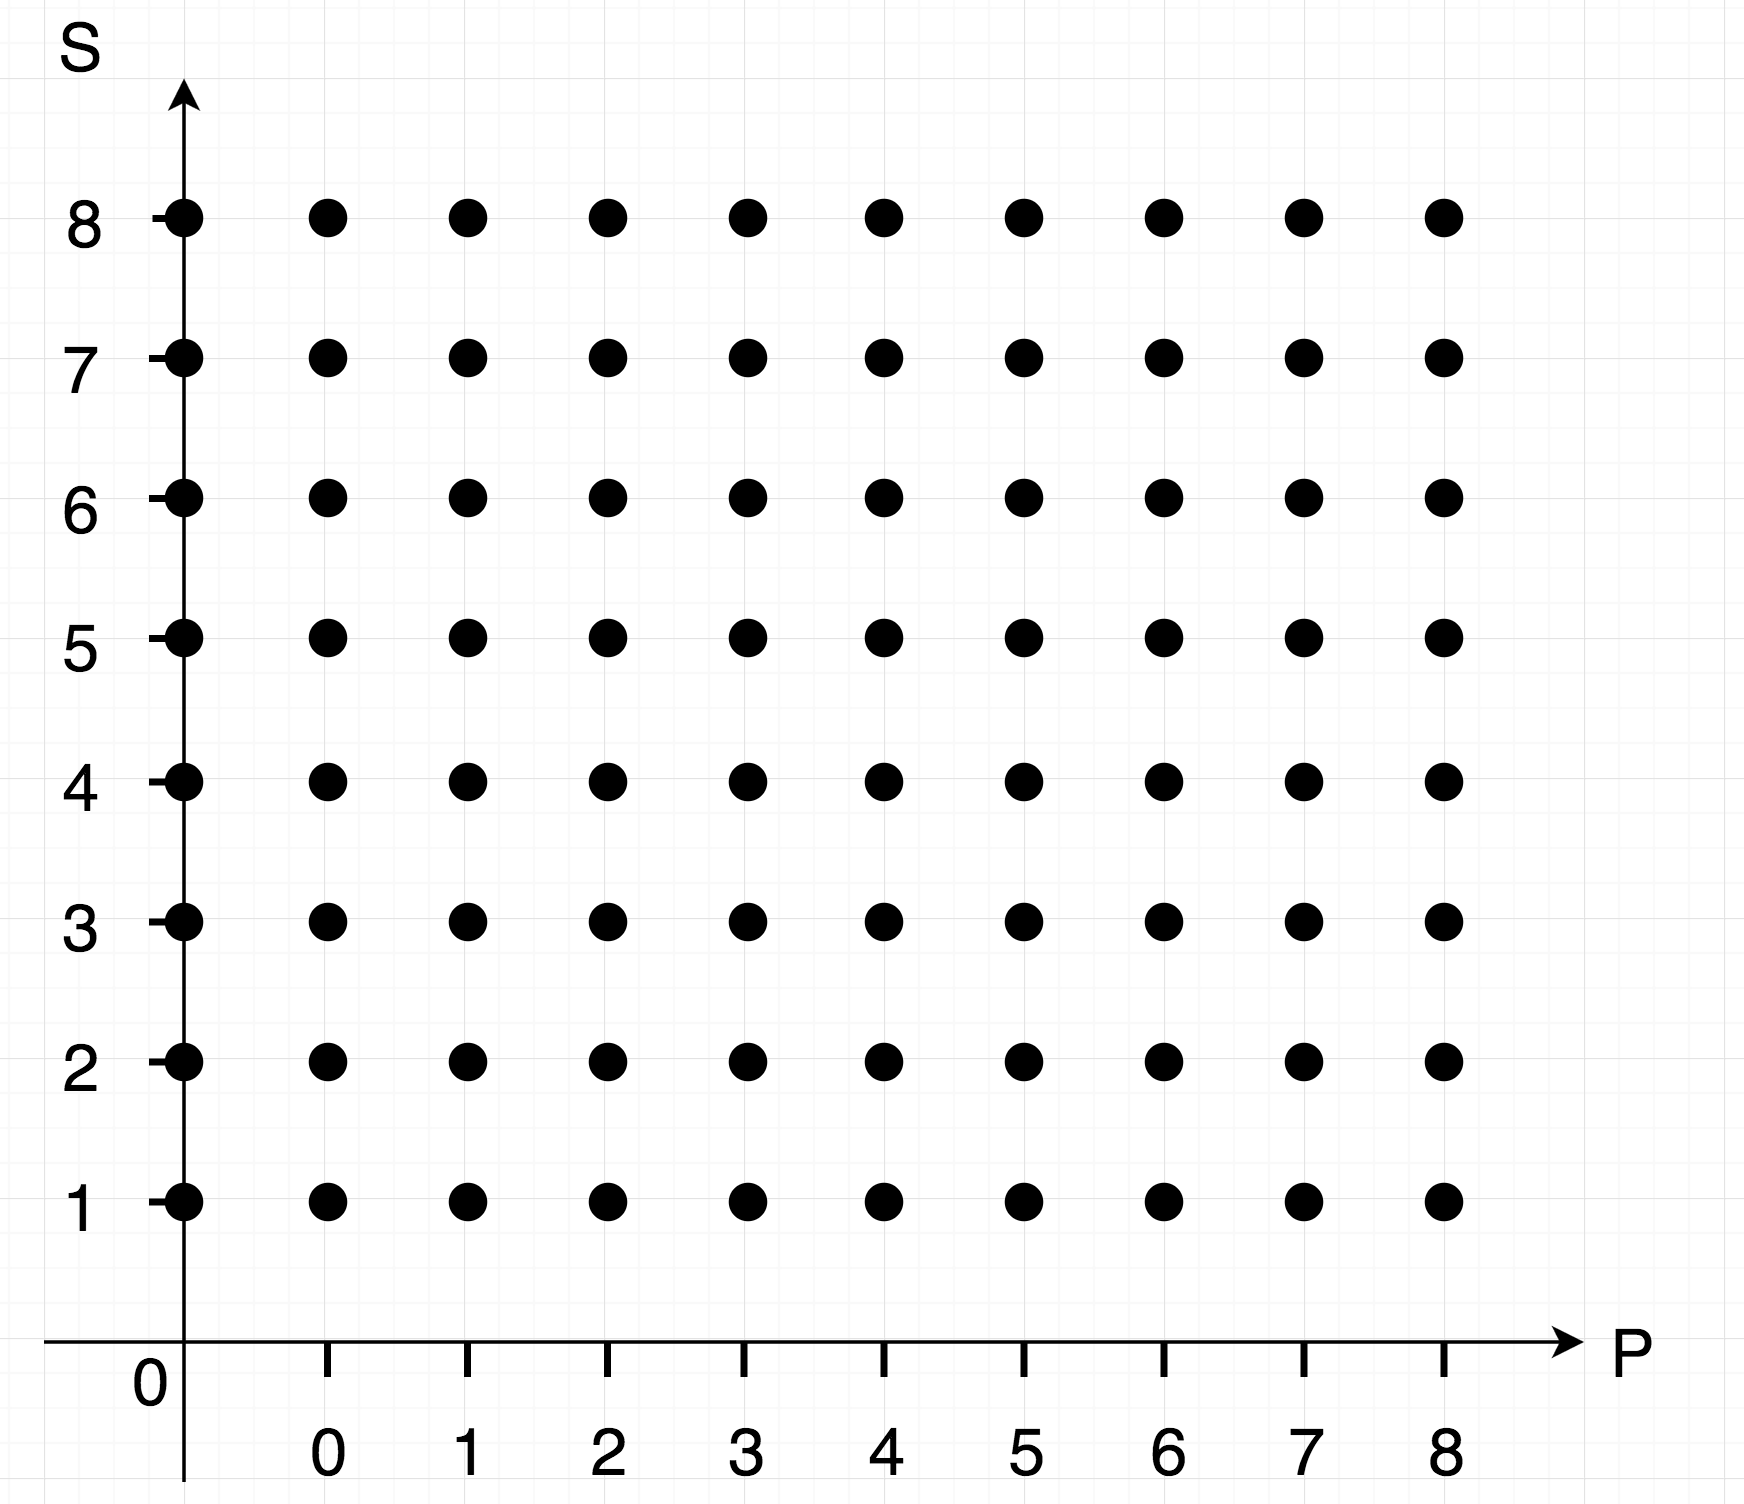
\includegraphics[scale=0.15]{images/2}

\paragraph{The dots are pairs (p,q) w/ $q \neq 0 \ p,q \in \mathbb{Z}$, which form a lattice. We can use the snake trick from the theorem to show that the positive rational numbers $Q^{+} =  \lbrace \frac{p}{q} \in \mathbb{Q} \ | \ \frac{p}{q} > 0\rbrace$ are countably infinite.}
\paragraph{}

\begin{minipage}[b]{0.35\linewidth}
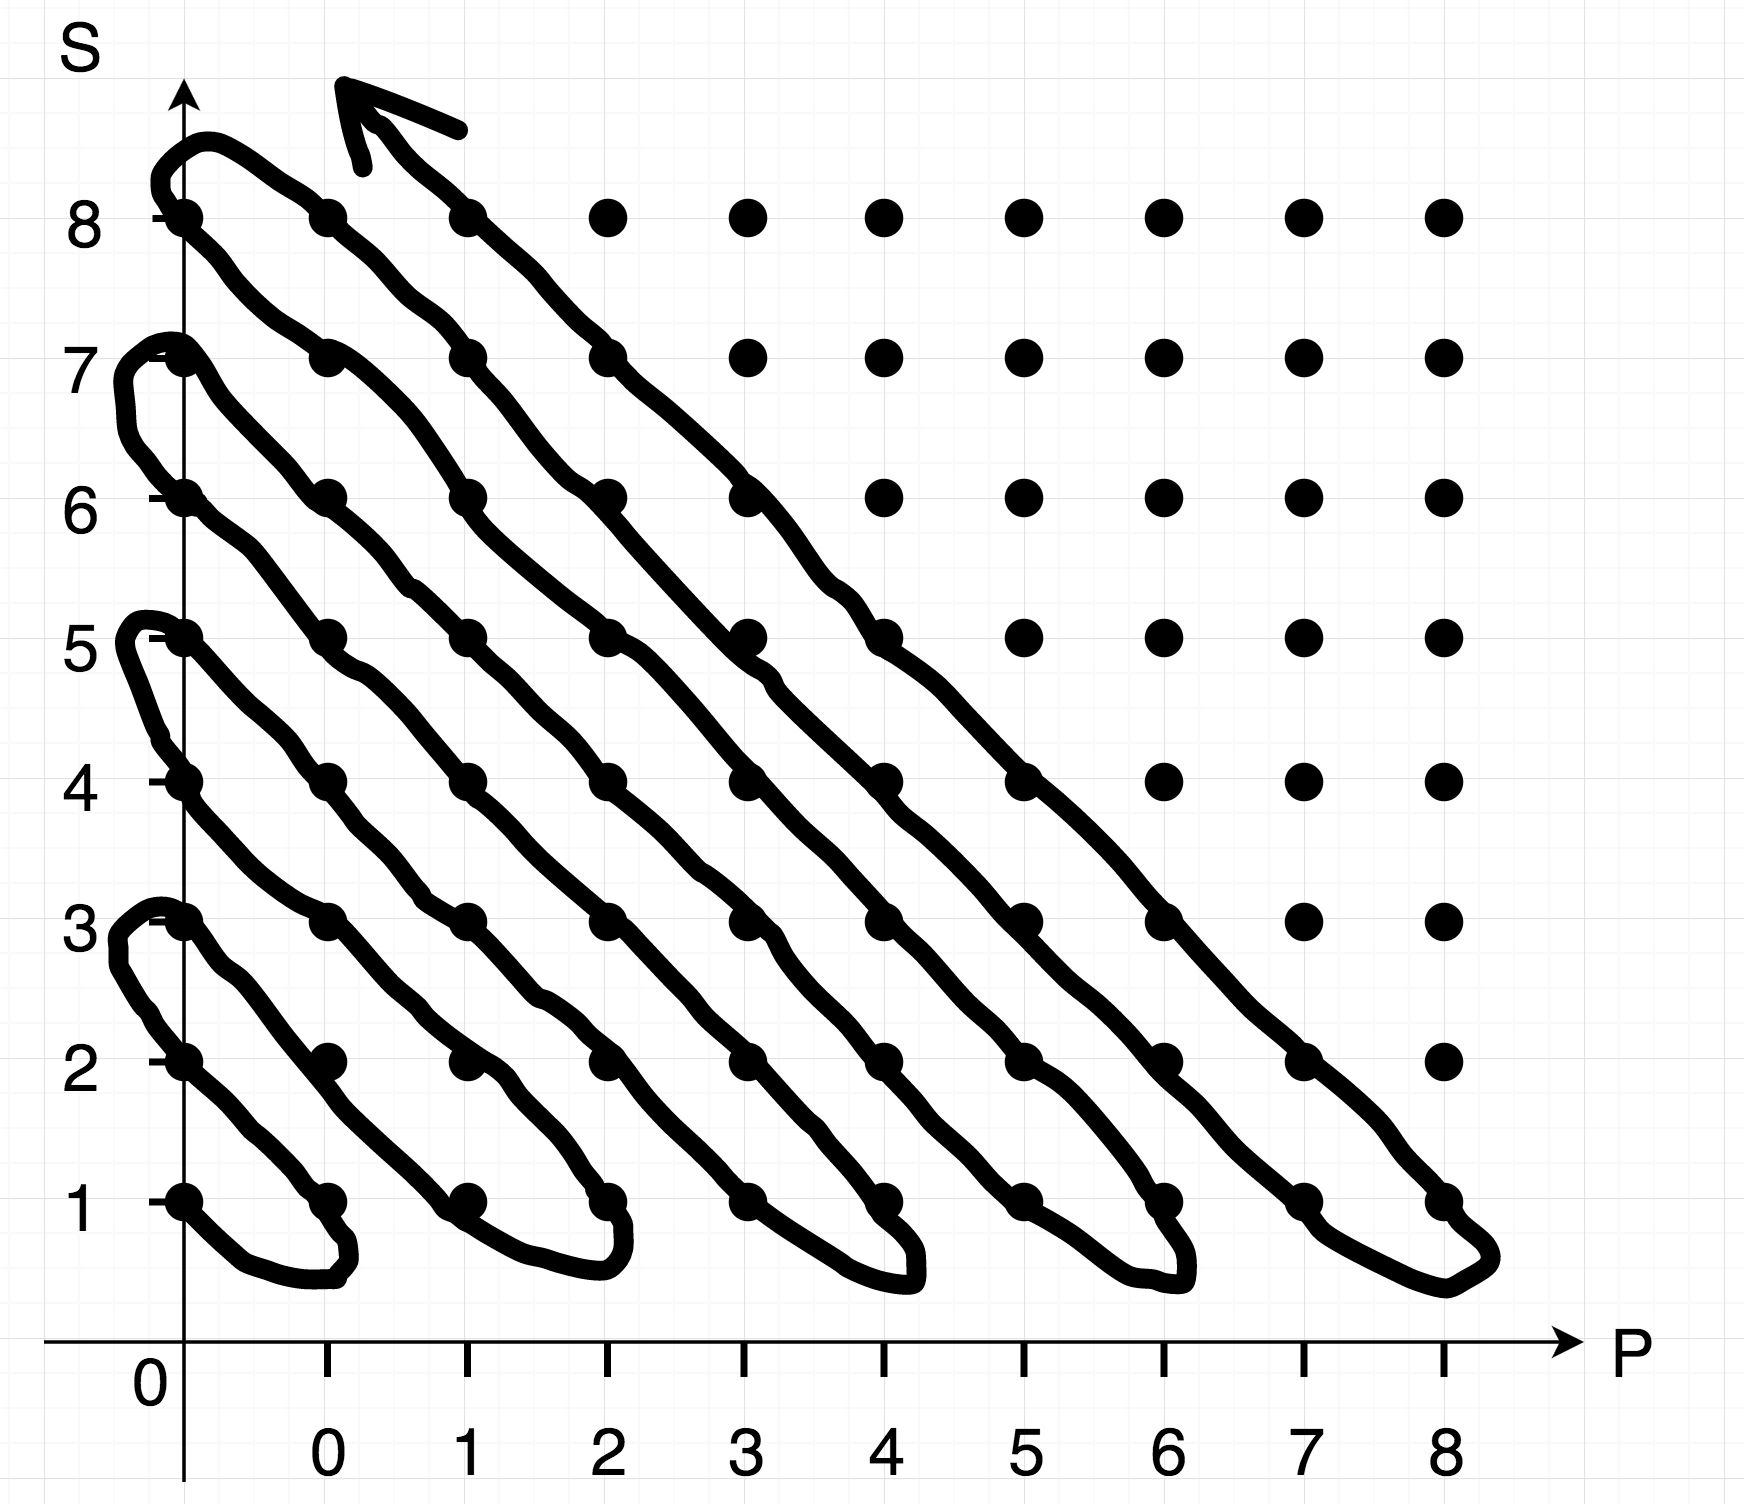
\includegraphics[scale=0.07]{images/3}
\end{minipage}
\hfill
\begin{minipage}[b]{0.65\linewidth}
\normalsize
Similarly we can show\newline $\mathbb{Q}^{-} = \lbrace \frac{p}{q} \in \mathbb{Q} \ | \ \frac{p}{q} > 0 \rbrace$ \newline is countably infinite.\newline
\linebreak
\linebreak
\linebreak
\end{minipage}

\paragraph{Then $\mathbb{Q} = \mathbb{Q}^{-} \cup \lbrace 0 \rbrace \cup \lbrace \mathbb{Q}^{+} \rbrace$ is countably infinite by Corollary 1.\newline 
Next, show that the set of sequences of 0's and 1's is uncountably infinite. We will use this result to show other sets are uncountably infinite.}

\paragraph{\underline{Theorum:} Let $A$ be the set of all sequences $s = \lbrace x_{1},x_{2},...\rbrace = \lbrace x_{n} \rbrace _{n = 1,2,3...}$ such that $x_{n} \in \lbrace 0,1 \rbrace \ \forall n \geq 1.$ Then $A$ is uncountably infinite}

\paragraph{\underline{Remark:} This result is proven via a clever construction, which is due to Georg Cantor (1845 - 1918). A very famous German mathematician who invented set theory. Cantor also came up with the diagonal argument (snake trick) we used to prove a countably infinite union of countably infinite sets is countably infinite, the idea that sizes of sets should be understood via bijections $(A \sim B \ $ for$ \ A,B $ sets$).$ As well as the notions of countably infinite and uncountably infinite.}

\paragraph{\underline{Proof:} Assume A is countable $\iff A = \lbrace s_{1},s_{2},...\rbrace$ ,where $s_{j} = \lbrace x_{n}^{j}\rbrace _{n = 1,2,...}$ for $x_{n}^{j} = 0$ or $x_{n}^{j} = 1$. We will now construct a sequence $s_{0}$ of $0's$ and $1's$ that cannot be in the enumeration $\lbrace s_{1},s_{2},...\rbrace$. Let $s_{0}$ be such that 
}\normalsize
\begin{equation}
 	 x_{j}^{0}=\begin{cases}
    1, & \text{if $x_{j}^{j} = 0$}.\\
    0, & \text{if $ x_{j}^{j} = 1 $}.
  \end{cases}
\end{equation}
\paragraph{In other words $s_{0}$ differs form each $s_{j}$ in the $j^{th}$ element \newline $\Longrightarrow s_{0} \notin \lbrace s_{1}, s_{2},... \rbrace$, but $s_{0}$ is a sequence of 0's and 1's $\Rightarrow s_{0} \in A \Rightarrow\!\Leftarrow$}
\end{document}